%LTeX: language=es

\documentclass[floatsintext,longtable]{apa7}
\usepackage[utf8]{inputenc}
\usepackage[backend=biber,style=ieee]{biblatex}
\usepackage[spanish]{babel}
\usepackage{csquotes}
\usepackage[utf8]{inputenc}
\usepackage[T1]{fontenc}
\usepackage{float}
\usepackage{graphicx}
\usepackage{makecell}
\usepackage{multirow}
\usepackage{parskip}
\usepackage{subcaption}
% \usepackage[margin=1cm]{geometry}
\usepackage{caption}
\setlength{\parskip}{1em} % Adjust the value as needed
\setlength{\parindent}{2em}
\captionsetup[table]{name=Tabla}

\addbibresource{references.bib}
\addbibresource{references_manual.bib}
\title{Exploración de filtros espaciales y morfológicos en escenarios reales }

\authorsnames[1,1,1,1]{Andrés Vásquez-Restrepo, Carlos Alberto Francisco Aguilar Chamochumbi, Federico Ezequiel Capdeville, Miguel Ángel Osorio Sánchez}
\authorsaffiliations{{Universidad Internacional de la Rioja}}
\course{Visión Artificial}
\professor{Alexandre Pérez Reina}
\date{Enero 2025}
\shorttitle{Artículo}
\leftheader{Visión Artificial}
\journal{Visión Artificial}
\duedate{Enero 2025}
\abstract{
    %LTeX: language=es
Este trabajo explora la aplicación de filtros espaciales y morfológicos en diversos escenarios de procesamiento de imágenes, incluyendo imágenes satelitales, médicas e industriales. Se implementaron y evaluaron técnicas para la detección de 9 casos de estudio de interes comercial. Los resultados demuestran la eficacia de estos métodos en la delimitación precisa de áreas de interés y en la identificación de características específicas en diferentes tipos de imágenes. En particular, se logró una detección precisa de la huella urbana en imágenes satelitales y una segmentación efectiva de melanomas en imágenes dermatológicas. Aunque se observaron algunas limitaciones, como la ocasional clasificación errónea en ciertas condiciones, los métodos demostraron ser robustos y efectivos en general. Este estudio resalta la continua relevancia de los filtros espaciales y morfológicos en el procesamiento moderno de imágenes, sugiriendo su potencial como complemento valioso a técnicas más avanzadas como el aprendizaje profundo. Se concluye que estas técnicas clásicas siguen siendo herramientas poderosas en el análisis de imágenes y se recomienda su integración con métodos más recientes para desarrollar soluciones aún más efectivas en futuras aplicaciones.}
\keywords{Filtros espaciales, Filtros morfológicos, Visión Artificial}
\begin{document}
\maketitle
\section{Introducción}
%LTeX: language=es

El procesamiento de imágenes digitales juega un papel crucial en diversos campos, incluyendo el análisis de imágenes médicas y satelitales. Aunque los métodos de aprendizaje profundo han ganado prominencia, las técnicas tradicionales de procesamiento de imágenes, como los operadores morfológicos y espaciales, siguen siendo herramientas valiosas.

Los operadores morfológicos, fundamentados en la teoría de conjuntos y la topología algebraica, demuestran una utilidad particular en el procesamiento de imágenes binarias y en escala de grises, facilitando la transformación de estructuras geométricas y topológicas en las matrices de píxeles \autocite{gonzalezDigitalImageProcessing2018}. 

En contraste, los operadores espaciales se concentran en el análisis de las relaciones entre píxeles adyacentes en el dominio espacial, resultando cruciales para operaciones como la detección de discontinuidades, la atenuación de ruido estocástico y la optimización del rango dinámico. \autocite{gonzalezDigitalImageProcessing2018}

En este paradigma, los operadores morfológicos y espaciales desempeñan un rol fundamental en las etapas de preprocesamiento y análisis de estas representaciones matriciales. Investigaciones empíricas extensivas han corroborado que la integración de algoritmos de preprocesamiento y posprocesamiento en un marco de inteligencia artificial puede incrementar significativamente la eficacia de los modelos computacionales en comparación con arquitecturas neuronales aisladas \autocite{salviImpactPrePostimage2021}.

\paragraph{Imágenes Médicas} En el ámbito médico, los operadores morfológicos se han aplicado eficazmente para la detección de bordes y la reducción de ruido. Por ejemplo, Peng L (2020) propuso un algoritmo de gradiente morfológico mejorado combinado con momentos de Zernike para la detección de bordes subpíxel en imágenes médicas \autocite{liu2020improvement}.

Los operadores espaciales, como Sobel y Canny, son ampliamente utilizados en el procesamiento de imágenes médicas. Xiao X M (2019) destacó la importancia de aplicar el operador Sobel a la detección de bordes en imágenes médicas \autocite{xiao2019application}. Qian (2019) propuso un algoritmo mejorado de detección de bordes Canny que incorpora filtrado de mediana adaptativo, operadores Sobel y el método de Otsu \autocite{qian2019medical}.\\



\paragraph{Imágenes Satelitales} En el campo de las imágenes satelitales, los operadores morfológicos y espaciales también desempeñan un papel crucial. Son particularmente útiles en áreas como la estimación del cambio climático global, la detección de cambios en la cobertura terrestre, el monitoreo ambiental como parte de la gestión de desastres, el desarrollo urbano y territorial, y la seguridad, entre otros \autocite{chang2017flexible}.

Los operadores espaciales, como el Sobel, se utilizan en imágenes satelitales para la detección de bordes, lo cual es fundamental en la identificación de límites entre diferentes tipos de terreno o estructuras. El operador Canny, conocido por su eficacia en la detección de bordes en presencia de ruido, se ha aplicado en el análisis de imágenes satelitales para la detección de características lineales como carreteras y ríos \autocite{abrahamEdgeDetectionSatellite2021}.

Así mismo, la segmentación es fundamental para dividir las imágenes en regiones significativas. Grinias et al. desarrollaron un método de segmentación basado en campos aleatorios de Markov y clasificación no supervisada, particularmente eficaz para la detección de edificios y carreteras en áreas periurbanas \autocite{grinias2016mrf}.\\



\paragraph{Industria} En la industria, los operadores morfológicos y espaciales se utilizan en aplicaciones como la inspección de calidad, la detección de defectos y la clasificación de productos. Por ejemplo, en la inspección de calidad de productos, los operadores morfológicos se utilizan para la detección de bordes y la segmentación de objetos, mientras que los operadores espaciales se utilizan para la detección de características específicas y detección de objetos  \autocite{demantPositioning2013,demantOverviewSegmentation2013,demantMarkIdentification2013}.

Por otro lado, la mejora de imagen es crucial para aumentar la calidad visual y la interpretabilidad de las imágenes. Singh et al. Propusieron un marco innovador de enmascaramiento de orden fraccionario con corrección gamma ponderada de manera óptima. Este método demostró una mejora significativa en el contraste y la preservación de detalles en imágenes \autocite{singh2017novel}.

La elección del operador puede impactar significativamente la velocidad y precisión del análisis, lo cual es crucial tanto en aplicaciones médicas como en el procesamiento de imágenes satelitales. En ambos campos, la integración de estas técnicas tradicionales con enfoques de aprendizaje profundo a menudo conduce a un rendimiento mejorado \autocite{asokanMachineLearningBased2019}.

Este estudio se orienta a la realización de un análisis comparativo exhaustivo de diversos operadores morfológicos y espaciales, evaluando su aplicabilidad y rendimiento en múltiples escenarios de análisis de imágenes satelitales y médicas, con énfasis en la cuantificación de métricas de desempeño y eficiencia algorítmica.

\section{Materiales y métodos}
\begin{figure*}[t]
    \centering
    \begin{tabular}{ccc}
        \subcaptionbox{\label{fig:a}}{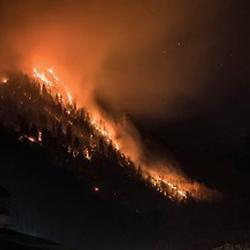
\includegraphics[width=3cm ]{./figures/drive/abc003.jpg}} &
        \subcaptionbox{\label{fig:b}}{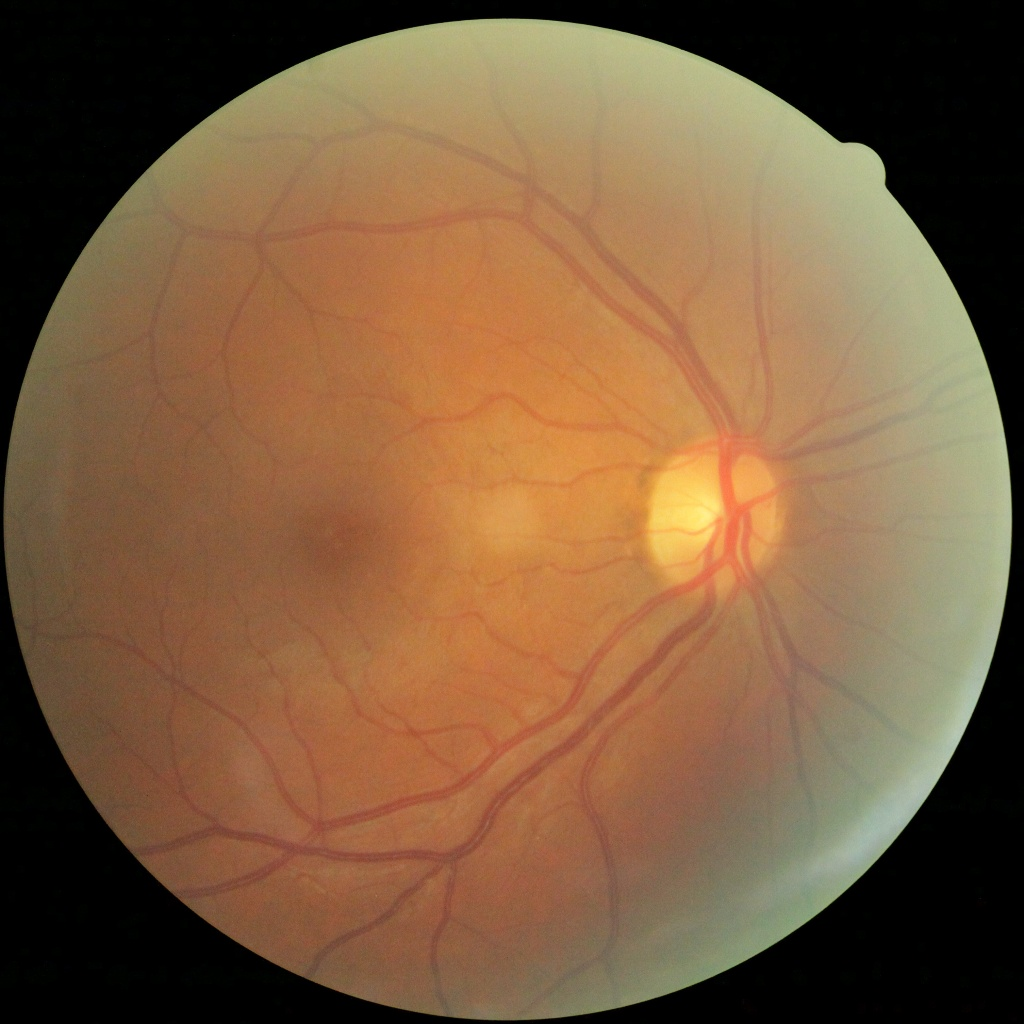
\includegraphics[width=3cm ]{./figures/drive/52_right.jpeg}} &
        \subcaptionbox{\label{fig:c}}{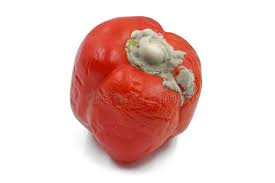
\includegraphics[width=3cm ]{./figures/drive/rottenPepper(93).jpg}} \\
        \subcaptionbox{\label{fig:d}}{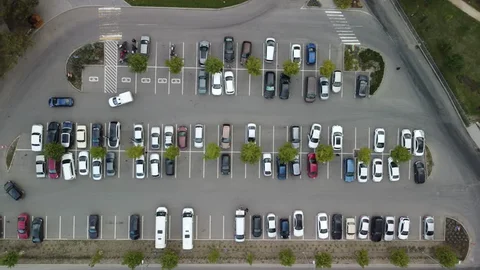
\includegraphics[width=3cm]{./figures/drive/parking_lot.png}} &
        \subcaptionbox{\label{fig:e}}{\includegraphics[width=3cm]{./figures/drive/Imagen_Satelital.png}} &
        \subcaptionbox{\label{fig:f}}{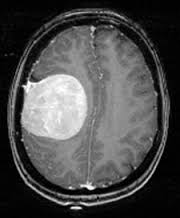
\includegraphics[width=3cm]{./figures/drive/Imagen_Medicina.jpg}} \\
        \subcaptionbox{\label{fig:g}}{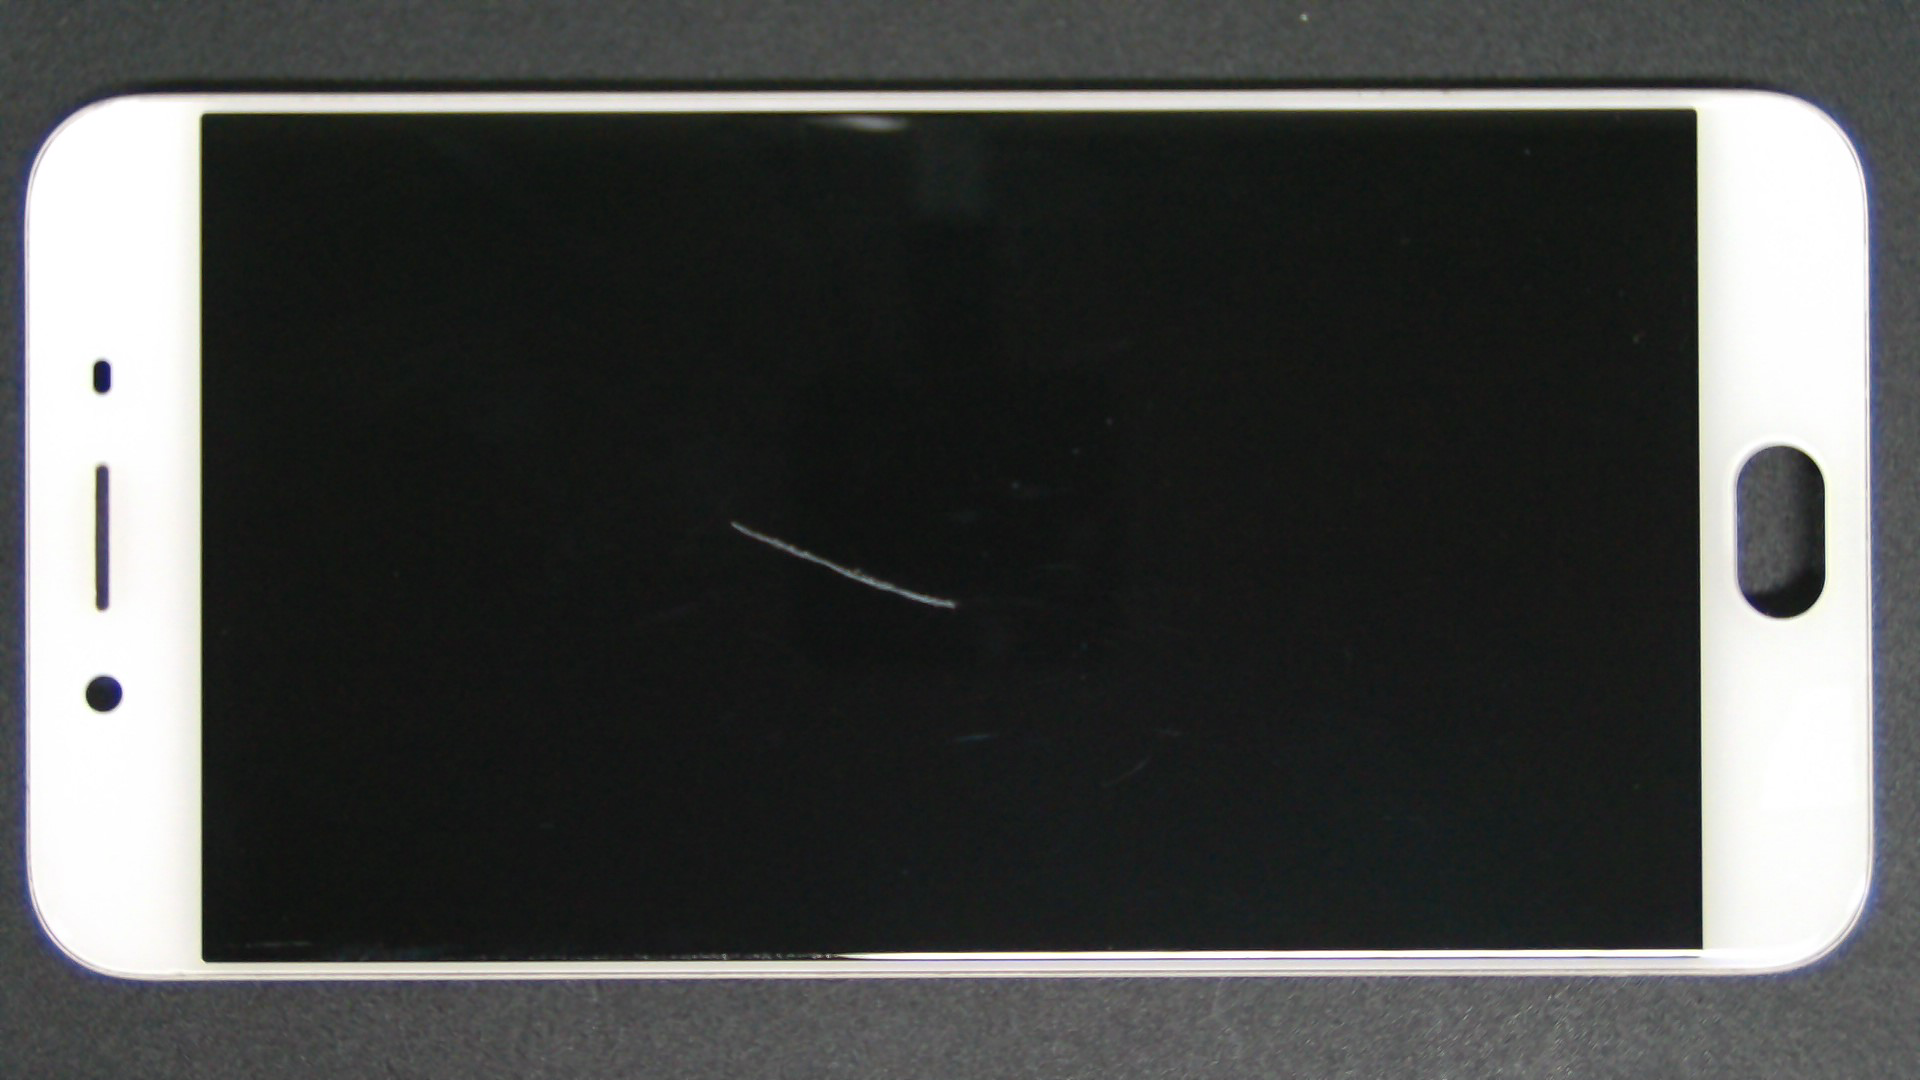
\includegraphics[width=3cm]{./figures/drive/Scr_0002.jpg}} &
        \subcaptionbox{\label{fig:h}}{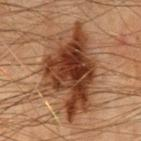
\includegraphics[width=3cm]{./figures/drive/melanoma_raw.jpg}} &
        \subcaptionbox{\label{fig:i}}{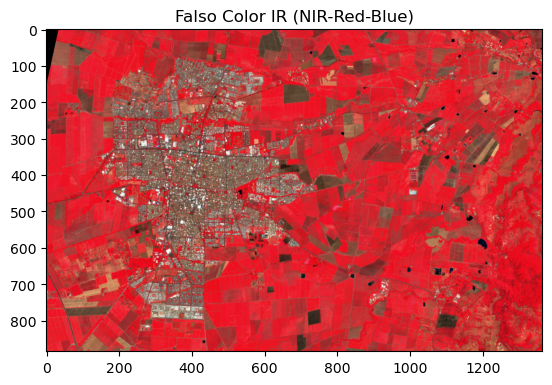
\includegraphics[width=3cm]{./figures/drive/palmira_nir.png}} \\
    \end{tabular}
    \caption{Imágenes originales utilizadas en el estudio de operadores morfológicos y espaciales.
    \subref{fig:a} Incendio Forestal \autocite{WildfireDetectionImage}.
    \subref{fig:b} Retinopatía Diabética \autocite{DiabeticRetinopathyResized}.
    \subref{fig:c} Inspección de Calidad en frutas \autocite{FruitVegetableDisease}
    \subref{fig:d} Estacionamiento \autocite{pklot-raw_dataset}.
    \subref{fig:e} Imagen Satelital de un Puerto \autocite{ShipsSatelliteImagery}.
    \subref{fig:f} Imagen Médica de un Tumor en el Cerebro \autocite{BrainMRIImages}.
    \subref{fig:g} Defectos de Pantalla en un celular \autocite{MobilePhoneDefect}.
    \subref{fig:h} Imagen Médica de un Melanoma \autocite{ISICInternationalSkin}.
    \subref{fig:i} Imagen Satelital de Palmira, Colombia en Falso Color IR  \autocite{sinergiseFalseColorInfrared}.
    }
    \label{fig:9x9}
\end{figure*}
%LTeX: language=es
\subsection{Entorno de desarrollo}
Para la implementación de los operadores morfológicos y espaciales, se ha utilizado el lenguaje de programación Python en su versión 3.12.X, junto con las bibliotecas NumPy \autocite{harris2020array}, OpenCV \autocite{opencv_library} y Scikit-image \autocite{van2014scikit}. Estas ofrecen una amplia gama de funciones y métodos para la manipulación de matrices y la aplicación de operadores morfológicos y espaciales.

\subsection{Casos de estudio}

\paragraph{Detección de Incendios Forestales} La detección temprana de incendios forestales es crucial para minimizar los daños ambientales y económicos.  El objetivo del presente caso es poder detectar en la imagen, señales de humo que indiquen un incendio eminente. La Figura \ref{fig:a} muestra la imagen original utilizada en este caso de estudio \autocite{WildfireDetectionImage}.

El proceso de análisis de imagen propuesto comprende una secuencia de operaciones que incluyen: 
\begin{seriate}

\item un realce de contraste mediante multiplicación. 

\item Posteriormente, se efectúa una conversión a escala de grises para facilitar las transformaciones matemáticas subsiguientes.

\item Se aplican operaciones morfológicas para la reducción de ruido, seguidas de una dilatación para acentuar los contornos.

\item El proceso continúa con la eliminación de contornos secundarios, preservando únicamente el contorno principal.

\item Finalmente, se extrae el contorno dilatado y se fusiona con la imagen original para obtener la representación final del objeto de interés. 
\end{seriate}

\paragraph{Detección de Retinopatía Diabética} La retinopatía diabética es una complicación de la diabetes que afecta los vasos sanguíneos de la retina. La detección temprana de esta enfermedad es fundamental para prevenir la pérdida de visión. En este caso de estudio, se busca identificar la presencia de microaneurismas en la retina, que son un indicador temprano de retinopatía diabética. La Figura \ref{fig:b} muestra la imagen original utilizada en este caso de estudio \autocite{DiabeticRetinopathyResized}.

Inicialmente, 
\begin{seriate}
    
    \item se convierte a escala de grises para facilitar las operaciones matemáticas subsiguientes. 
    
    \item Se aplica una ecualización de histograma para mejorar el contraste, redistribuyendo uniformemente las intensidades de los píxeles y realzando los detalles, especialmente en áreas oscuras o de bajo contraste. 
    
    \item A continuación, se realiza una segmentación utilizando el algoritmo Canny para detección de bordes. 
    
    \item Se implementa una operación morfológica de apertura con un kernel tipo elipse de \( 5x5 \) para reducir el ruido en la imagen resultante y centrarse en las zonas de potencial daño vascular. 
    
    \item Finalmente, se fusiona la imagen procesada, convertida de nuevo a formato RGB, con la imagen original, aplicando una tonalidad de 3/7 para resaltar las áreas de interés.
\end{seriate}



\paragraph{Inspección de Calidad en Frutas} La inspección de calidad en frutas es un proceso crucial en la industria alimentaria para garantizar la seguridad y la calidad de los productos. En este caso de estudio, se busca identificar frutas podridas en una imagen de inspección de calidad. La Figura \ref{fig:c} muestra la imagen original utilizada en este caso de estudio \autocite{FruitVegetableDisease}.

\begin{seriate}

    
    \item Se parte de una conversión a escala de grises para simplificar el procesamiento y reducir la complejidad computacional, ya que la información de color no es esencial para la detección de anomalías estructurales.
    
    \item Se ajustan los valores de intensidad de los píxeles a un rango estándar, típicamente \( [0, 1] \). Esta operación mejora la consistencia entre diferentes imágenes y facilita el procesamiento posterior al establecer una escala uniforme.
    
    \item Se aplica un operador de gradiente (como Sobel o Prewitt) en la dirección horizontal. Este paso resalta los cambios abruptos de intensidad en el eje x, que pueden indicar bordes o anomalías en la superficie de la fruta.
    
    \item Similar al paso anterior, pero en la dirección vertical. La combinación de los gradientes \( x \) e \( y \) proporciona una representación completa de los cambios de intensidad en la imagen, crucial para detectar irregularidades en la textura de la fruta.
    
    \item Se binariza la imagen para resaltar las áreas de mayor cambio en intensidad, es decir, los bordes y las regiones con texturas anómalas.
    
    \item Finalmente, Fusión con la imagen original: La imagen procesada se combina con la original, permitiendo una visualización intuitiva de las áreas problemáticas en el contexto de la fruta completa.
    
    \end{seriate}

\paragraph{Detección de Automóviles en parqueadero} La detección de vehículos en estacionamientos es una tarea común en aplicaciones de monitoreo de tráfico y seguridad. En este caso de estudio, se busca identificar los vehículos en un estacionamiento a partir de una imagen aérea. La Figura \ref{fig:d} muestra la imagen original utilizada en este caso de estudio \autocite{pklot-raw_dataset}.

\begin{seriate}

   \item La imagen del parqueadero se transforma a escala de grises mediante para simplificar el procesamiento posterior.
    
    \item Se aplican dos operaciones morfológicas secuenciales: Apertura morfológica para eliminar pequeños objetos y suavizar contornos. Cierre morfológico  para cerrar pequeños huecos y conectar objetos cercanos.
    Estas operaciones ayudan a resaltar las formas de los vehículos y reducir el ruido.
    
    \item Se aplica un filtro gaussiano para reducir aún más el ruido y suavizar la imagen, preparándola para la detección de bordes.
    
    \item Se utiliza el algoritmo de Canny para detectar los bordes en la imagen, lo que ayuda a identificar los contornos de los vehículos.
    
    \item Se aplica un algoritmo de selección de contornos para identificar y extraer los contornos de los objetos en la imagen de bordes.
    
    \item Finalmente, los contornos detectados se dibujan sobre la imagen original, resaltando las áreas identificadas como vehículos.
    
    \end{seriate}

\paragraph{Detección de orillas en puertos} La detección de orillas en puertos es una tarea fundamental en aplicaciones de monitoreo marítimo y seguridad. En este caso de estudio, se busca identificar las orillas en una imagen satelital de un puerto. La Figura \ref{fig:e} muestra la imagen original utilizada en este caso de estudio \autocite{ShipsSatelliteImagery}.


\begin{seriate}

    \item La imagen satelital a color se convierte a escala de grises. 
    
    \item Se utiliza un operador tipo Sobel para identificar los contornos en la imagen y se binariza con dos diferentes umbrales pararesaltar los bordes.

    \item Se aplica una operación de dilatación morfológica utilizando un elemento estructural rectangular. Este paso ayuda a reforzar y conectar los bordes detectados, especialmente útil para delinear estructuras lineales como las orillas del puerto.
    
    \item Se implementa un filtro a nivel de codigo que elimina objetos pequeños basándose en su área. Este paso encuentra segmentos completos y estima su area para remover elementos no deseados como barcos pequeños o ruido que no forman parte de la estructura de la orilla o se aplica una operación de apertura morfológica (erosión seguida de dilatación) utilizando un elemento estructural rectangular. Se espera que esta transformación sea particularmente efectiva para eliminar objetos alargados como barcos, mientras preserva las estructuras más grandes y lineales de las orillas.
    
    \end{seriate}

\paragraph{Detección de Tumores Cerebrales} La detección temprana de tumores cerebrales es crucial para el tratamiento y la supervivencia de los pacientes. En este caso de estudio, se busca identificar tumores cerebrales en una imagen de resonancia magnética (MRI). La Figura \ref{fig:f} muestra la imagen original utilizada en este caso de estudio \autocite{BrainMRIImages}.

\begin{seriate}
\item Se convierte la imagen a escala de grises (Aunque la imagen original ya está en escala de grises, este paso es necesario para garantizar el canal correcto para las operaciones morfológicas y espaciales subsiguientes) y se normaliza a un rango de intensidad estándar \( [0, 1] \).

\item Se binariza la imagen con un umbral fijo de \( 0.65 \)

\item Se aplica una operación de dilatación morfológica utilizando un elemento estructural en forma de disco. Esta elección es crucial debido a la naturaleza generalmente redondeada de los tumores. La dilatación expande las regiones del tumor, lo que ayuda a resaltar la forma general del tumor, conectar áreas del tumor que podrían estar ligeramente separadas en la imagen original, aumentar el tamaño aparente del tumor para facilitar su identificación.

\item Después de la dilatación, se aplica una operación de apertura morfológica. Esta operación consiste en una erosión seguida de una dilatación, y tiene el efecto de eliminar pequeños objetos o protuberancias que podrían haber sido introducidos por la dilatación inicial,suavizar los contornos del tumor, eliminando irregularidades menores, preservar la forma general del tumor mientras se eliminan detalles finos que podrían ser ruido o artefactos.

\end{seriate}

\paragraph{Detección de defectos en pantallas de celulares} La detección de defectos en pantallas de celulares es una tarea común en la industria de la electrónica para garantizar la calidad de los productos. . La Figura \ref{fig:g} muestra la imagen original utilizada en este caso de estudio \autocite{MobilePhoneDefect}.

\begin{seriate}

    \item La imagen se convierte a escala de grises y se aplica una binarización simple con un valor de umbral de 0.2. Este paso convierte la imagen en blanco y negro, separando los objetos de interés (posiblemente ralladuras) del fondo.
    
    \item Se aplica una operación de erosión utilizando un elemento estructurante en forma de disco con radio 3. Con esta transformación se busca eliminar los posibles desperfectos para posteriormente ser resaltados con una operación Top-hat.
    
    \item La imagen erosionada se redimensiona para que coincida con las dimensiones de la imagen binaria original. Esto asegura que las operaciones subsiguientes se realicen en imágenes del mismo tamaño.
    
    \item Se realiza una operación Top-hat mediante una XOR bit a bit entre la imagen binaria original y la imagen erosionada redimensionada. Esta operación es particularmente útil para detectar elementos brillantes en un fondo oscuro o, en este caso, para resaltar las ralladuras.
    
\end{seriate}

\paragraph{Detección de Zonas Urbanas en Imágenes NIR-R-B}

El archivo es una imagen satelital de Sentinel 2 de la ciudad de Palmira, Valle del Cauca - Colombia, (Figura \ref{fig:h}).
A pesar de que este tipo de composición se utiliza para evaluar la salud en las plantas, podemos aprovechar el hecho de que en esta imagen se diferencia bastante bien entre las construcciones de la ciudad, terrenos baldíos y vegetación. Por lo que lo se usará para determinar la huella urbana de la ciudad de Palmira, incluyendo las construcciones de pequeños poblados a las afueras de la ciudad.

\begin{seriate}


    \item Se crea una composición usando las bandas NIR, roja y azul. Esta composición resalta la vegetación y ayuda a diferenciar áreas urbanas de vegetación.
    
    \item Cálculo del NDVI (Índice de Vegetación de Diferencia Normalizada. Se calcula para distinguir entre áreas con vegetación y áreas potencialmente urbanizadas. El NDVI es alto para vegetación y bajo para áreas construidas o suelo desnudo.
    
    \item Se crea una máscara binaria basada en el NDVI para una primera aproximación de áreas posiblemente urbanizadas.
    
    \item Se aplica un filtro morfológico de clausura para conectar estructuras urbanas contiguas y suavizar los bordes de la máscara.
    
    \item Se calcula la desviación estándar local en la banda roja para identificar áreas con alta heterogeneidad, característico de zonas urbanas.
    
    \item Se combina la máscara NDVI con la máscara de textura para refinar la detección de áreas urbanas.
    
    \item Se eliminan pequeños grupos de píxeles aislados mientras se preservan asentamientos pequeños mediante un filtrado por conectividad:.
    
    \item Se utiliza el gradiente morfológico para delinear los bordes de las áreas urbanas detectadas.
    
    \item Finalmente, se visualiza el resultado final superponiendo los bordes detectados sobre la imagen original.
    
    \end{seriate}



\paragraph{Detección de Melanoma} El melanoma es un tipo de cáncer de piel que puede ser mortal si no se detecta y trata a tiempo. En este caso de estudio, se busca identificar un melanoma en una imagen de piel. La Figura \ref{fig:i} muestra la imagen original utilizada en este caso de estudio \autocite{ISICInternationalSkin}.

\begin{seriate}

    \item Se aplica la operación morfológica de Black-hat seguida de inpainting para detectar y eliminar estructuras finas como el vello. Esto prepara la imagen para el análisis del melanoma sin interferencias.
    
    \item Se transforma la imagen de RGB a HSV para aprovechar la información de luminosidad (canal V) en la segmentación.
    
    \item Se realiza una umbralización del canal V utilizando el método de Otsu para obtener una máscara preliminar de la lesión.
    
    \item Se aplican operaciones de clausura (closing) y apertura (opening) para rellenar huecos y eliminar ruido en la máscara, respectivamente.
    
    \item Se identifica y selecciona la región conectada más grande, asumiendo que corresponde al melanoma, eliminando así pequeños artefactos o regiones no deseadas.
    
    \item Se superpone la máscara final sobre la imagen original para validar la segmentación del melanoma.
    
    \end{seriate}


% LTeX: language=es



\begin{figure*}[t]
    \centering
    % add file
    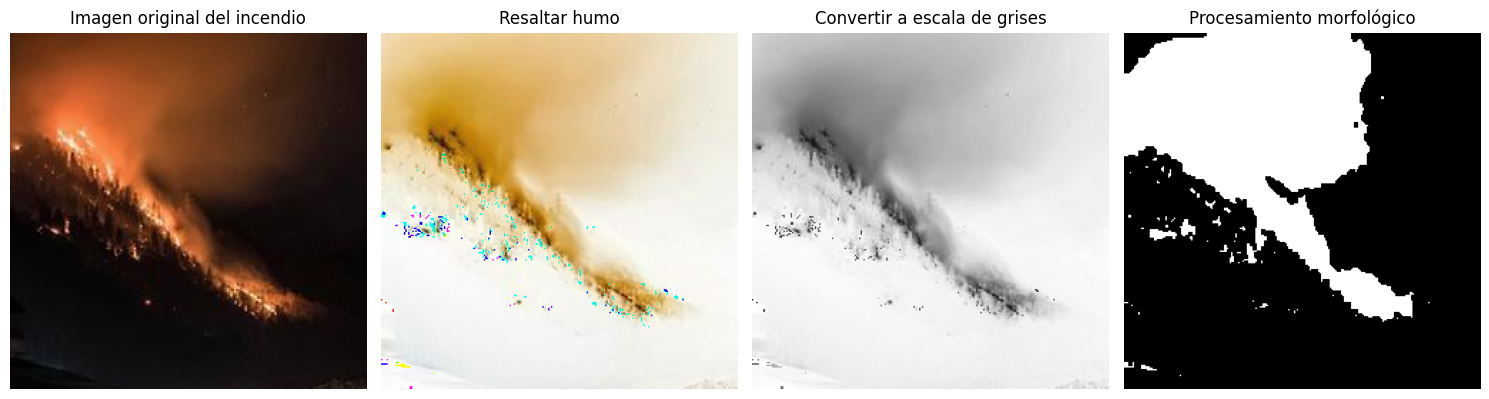
\includegraphics[height=0.15\textwidth]{./figures/drive/incendio.png}
    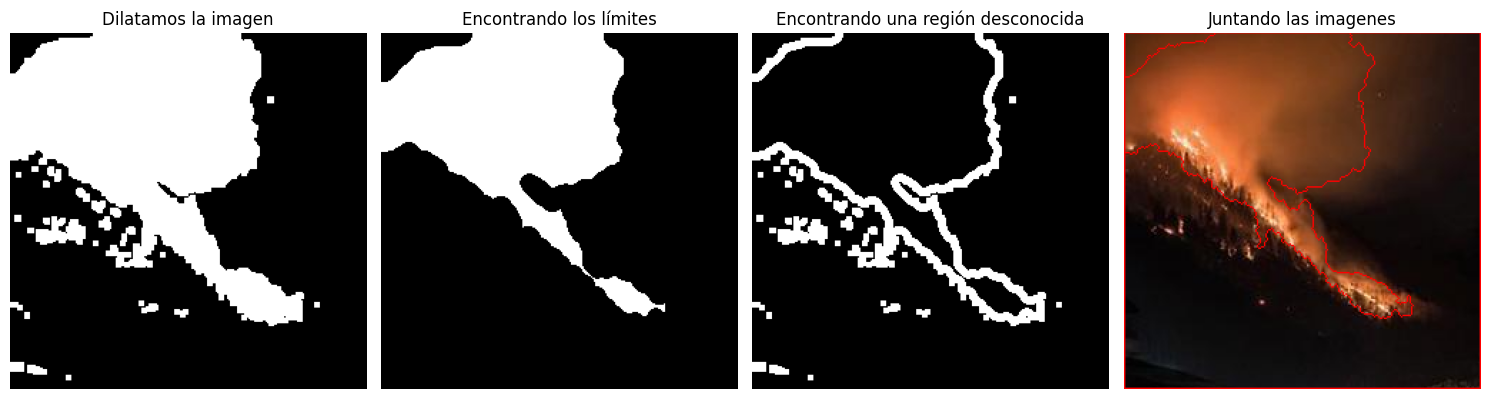
\includegraphics[height=0.15\textwidth]{./figures/drive/incendio_2.png}
    \caption{Resultados de la detección de incendios forestales.}
    \label{fig:incendio_results}
\end{figure*}

\begin{figure*}[t]
    \centering
    % add file
    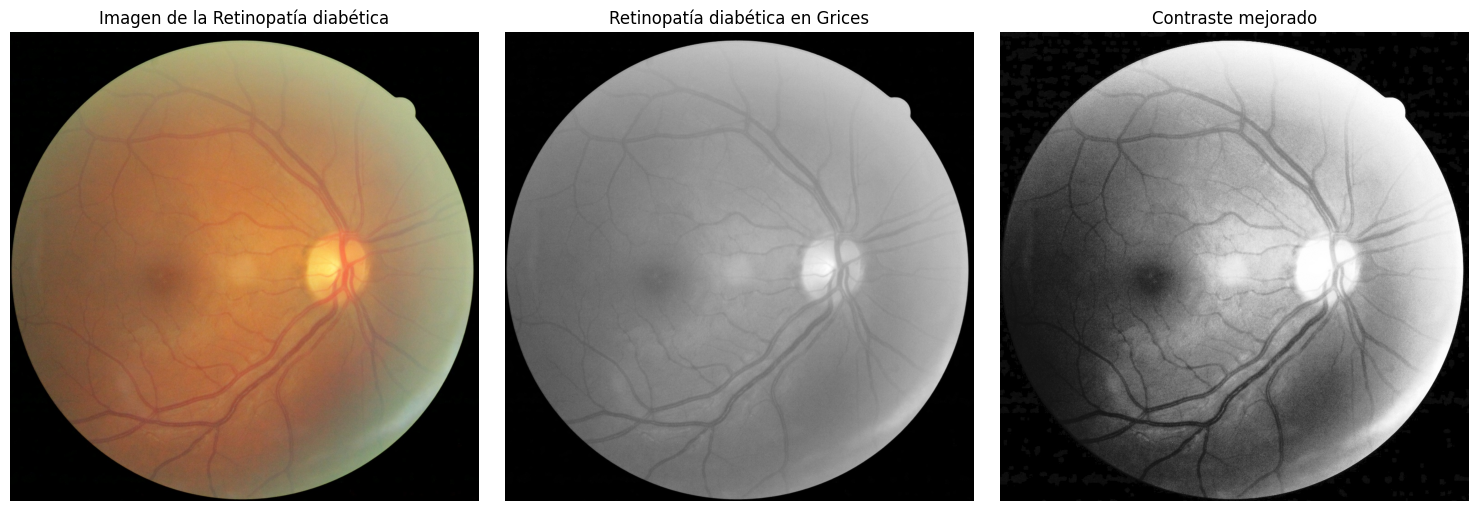
\includegraphics[height=0.15\textwidth]{./figures/drive/ojos.png}
    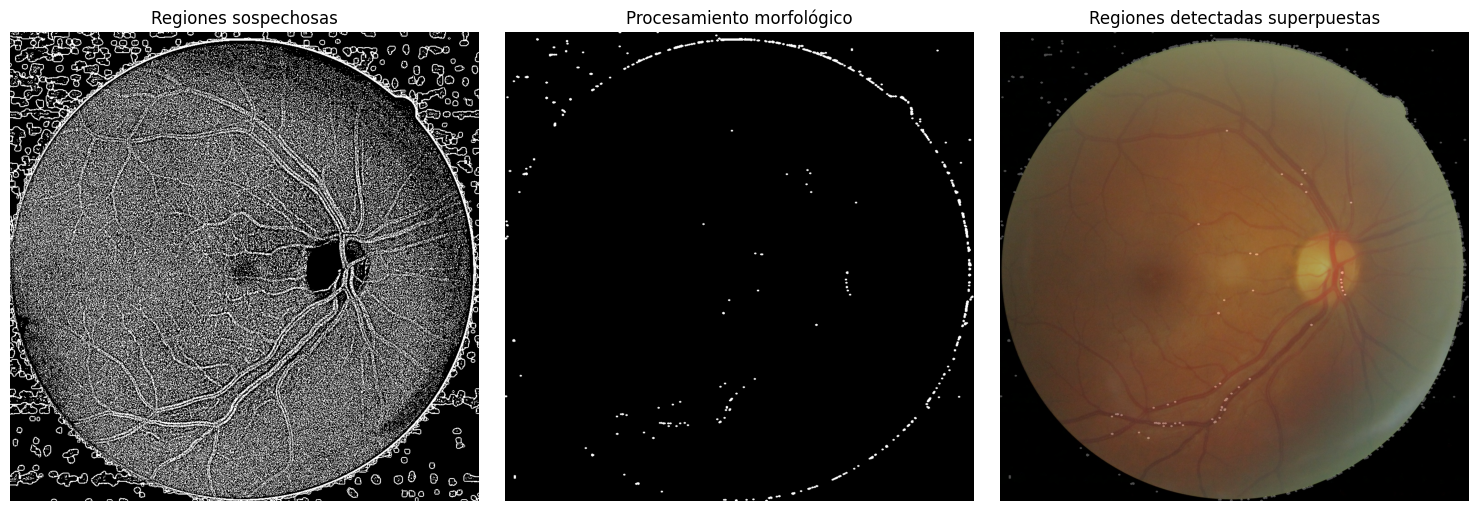
\includegraphics[height=0.15\textwidth]{./figures/drive/ojos_2.png}
    \caption{Resultados de la detección de retinopatía diabética.}
    \label{fig:retinopatia_results}
\end{figure*}

\begin{figure*}[t]
    \centering
    % add file
    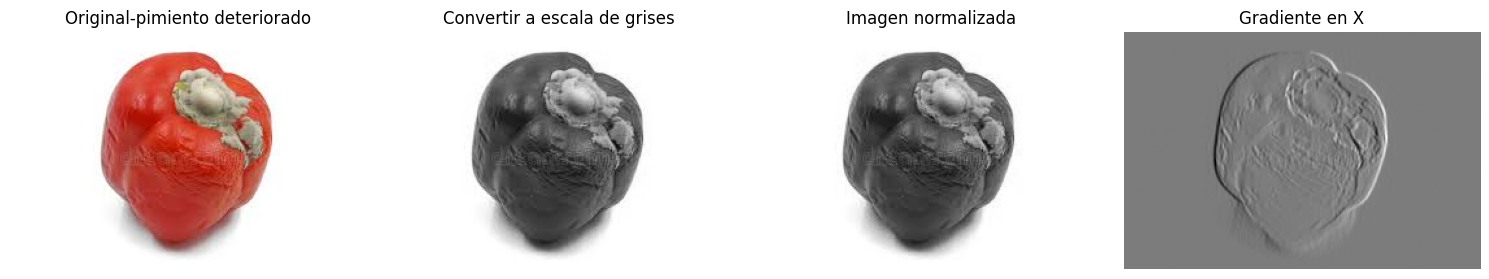
\includegraphics[height=0.15\textwidth]{./figures/drive/frutas.png}
    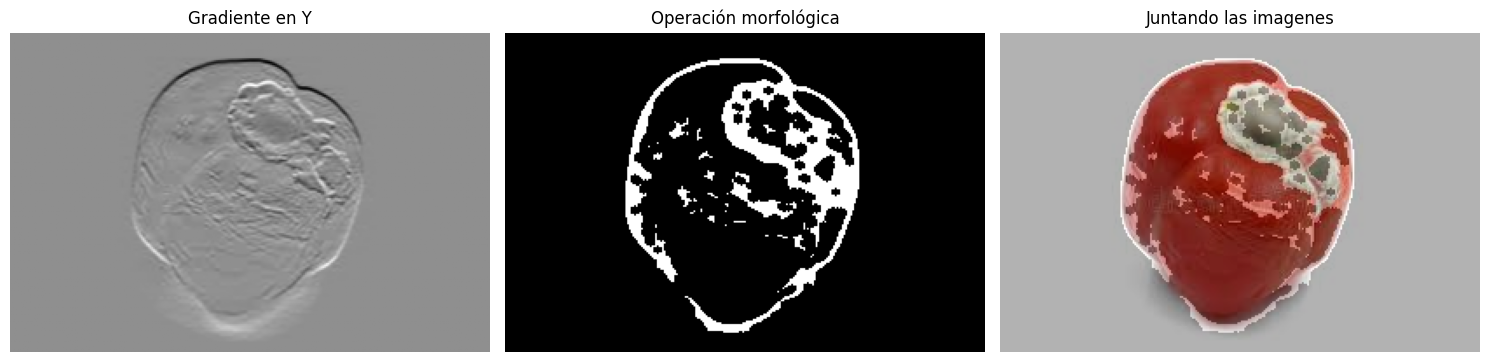
\includegraphics[height=0.15\textwidth]{./figures/drive/frutas_2.png}
    \caption{Resultados de la inspección de calidad en frutas.}
    \label{fig:frutas_results}
\end{figure*}

\begin{figure*}[t]
    \centering
    % add file
    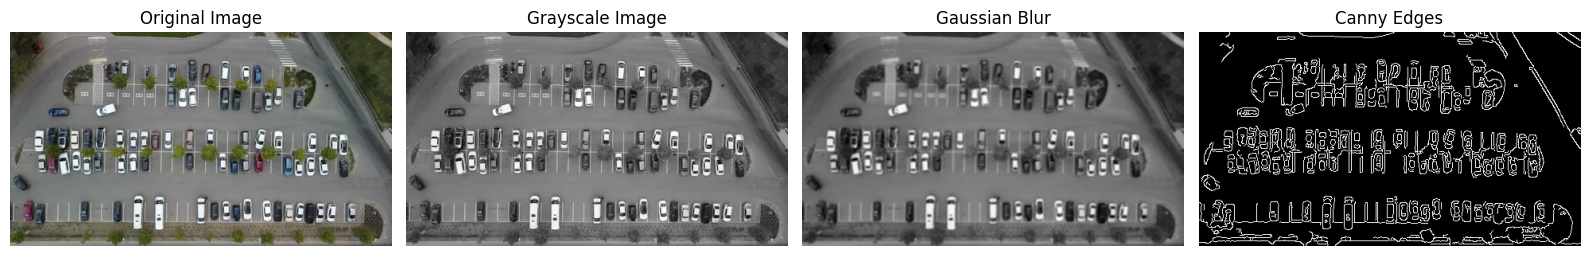
\includegraphics[height=0.15\textwidth]{./figures/drive/parqueadero.png}
    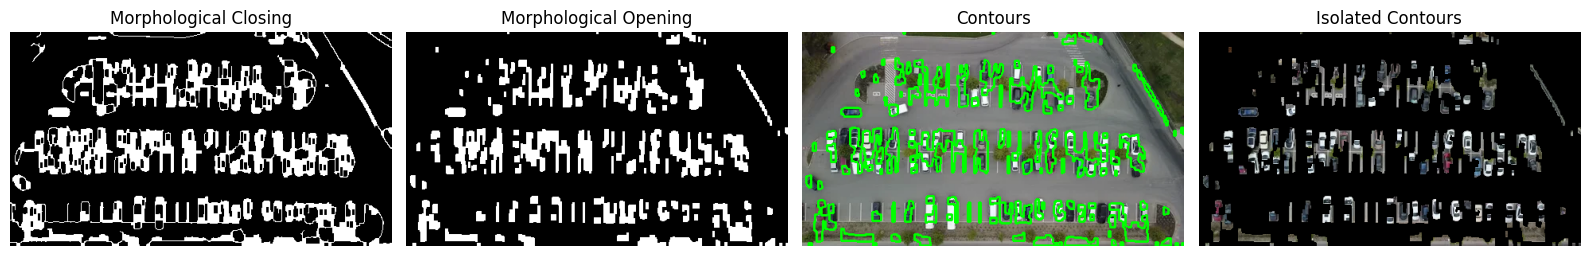
\includegraphics[height=0.15\textwidth]{./figures/drive/parqueadero_2.png}
    \caption{Resultados de la detección de automóviles en un parqueadero.}
    \label{fig:parqueadero_results}
\end{figure*}

\begin{figure*}[t]
    \centering
    % add file
    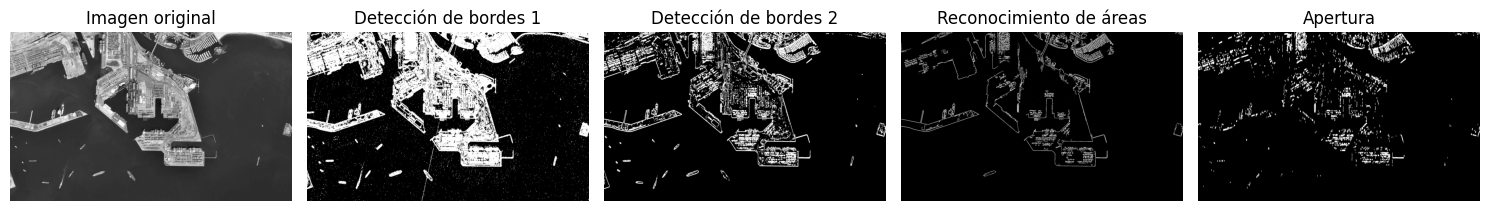
\includegraphics[width=1\textwidth]{./figures/drive/puerto.png}
    \caption{Resultados de la detección de orillas en puertos.}
    \label{fig:puerto_results}
\end{figure*}

\begin{figure*}[t]
    \centering
    % add file
    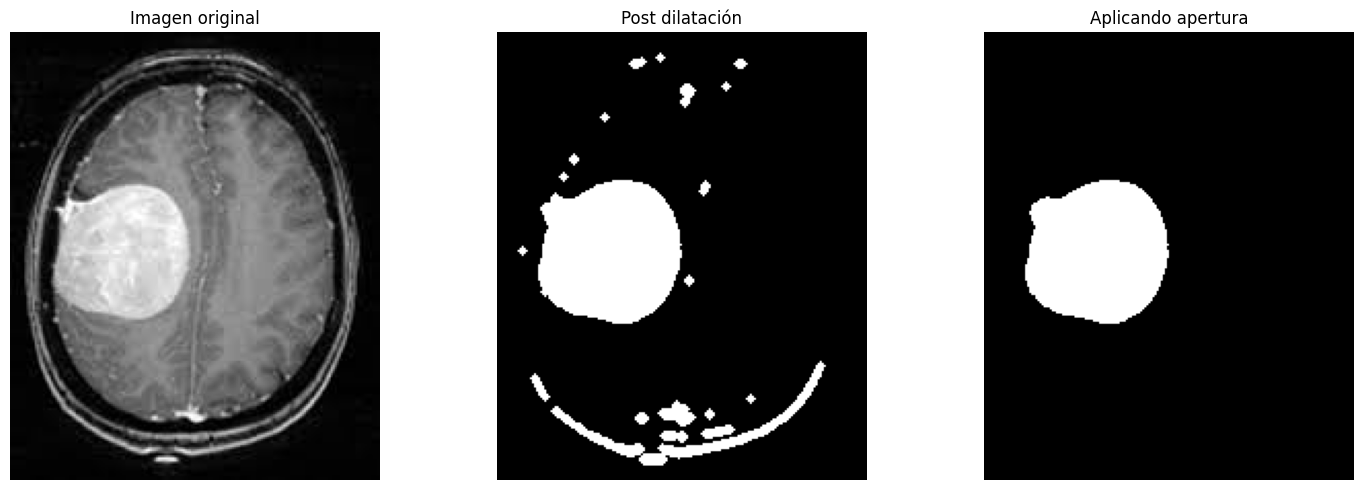
\includegraphics[height=0.30\textwidth]{./figures/drive/tumor.png}
    \caption{Resultados de la detección de tumores cerebrales.}
    \label{fig:tumor_results}
\end{figure*}

\begin{figure*}[t]
    \centering
    % add file
    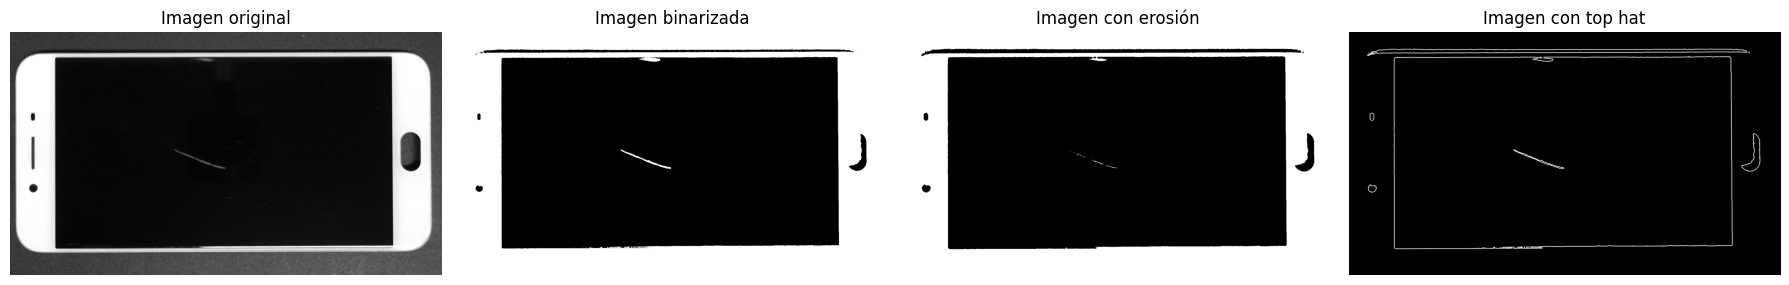
\includegraphics[width=1\textwidth]{./figures/drive/celulares.png}
    \caption{Resultados de la detección de defectos en pantallas de celulares.}
    \label{fig:celular_results}
\end{figure*}

\begin{figure*}[t]
    \centering
    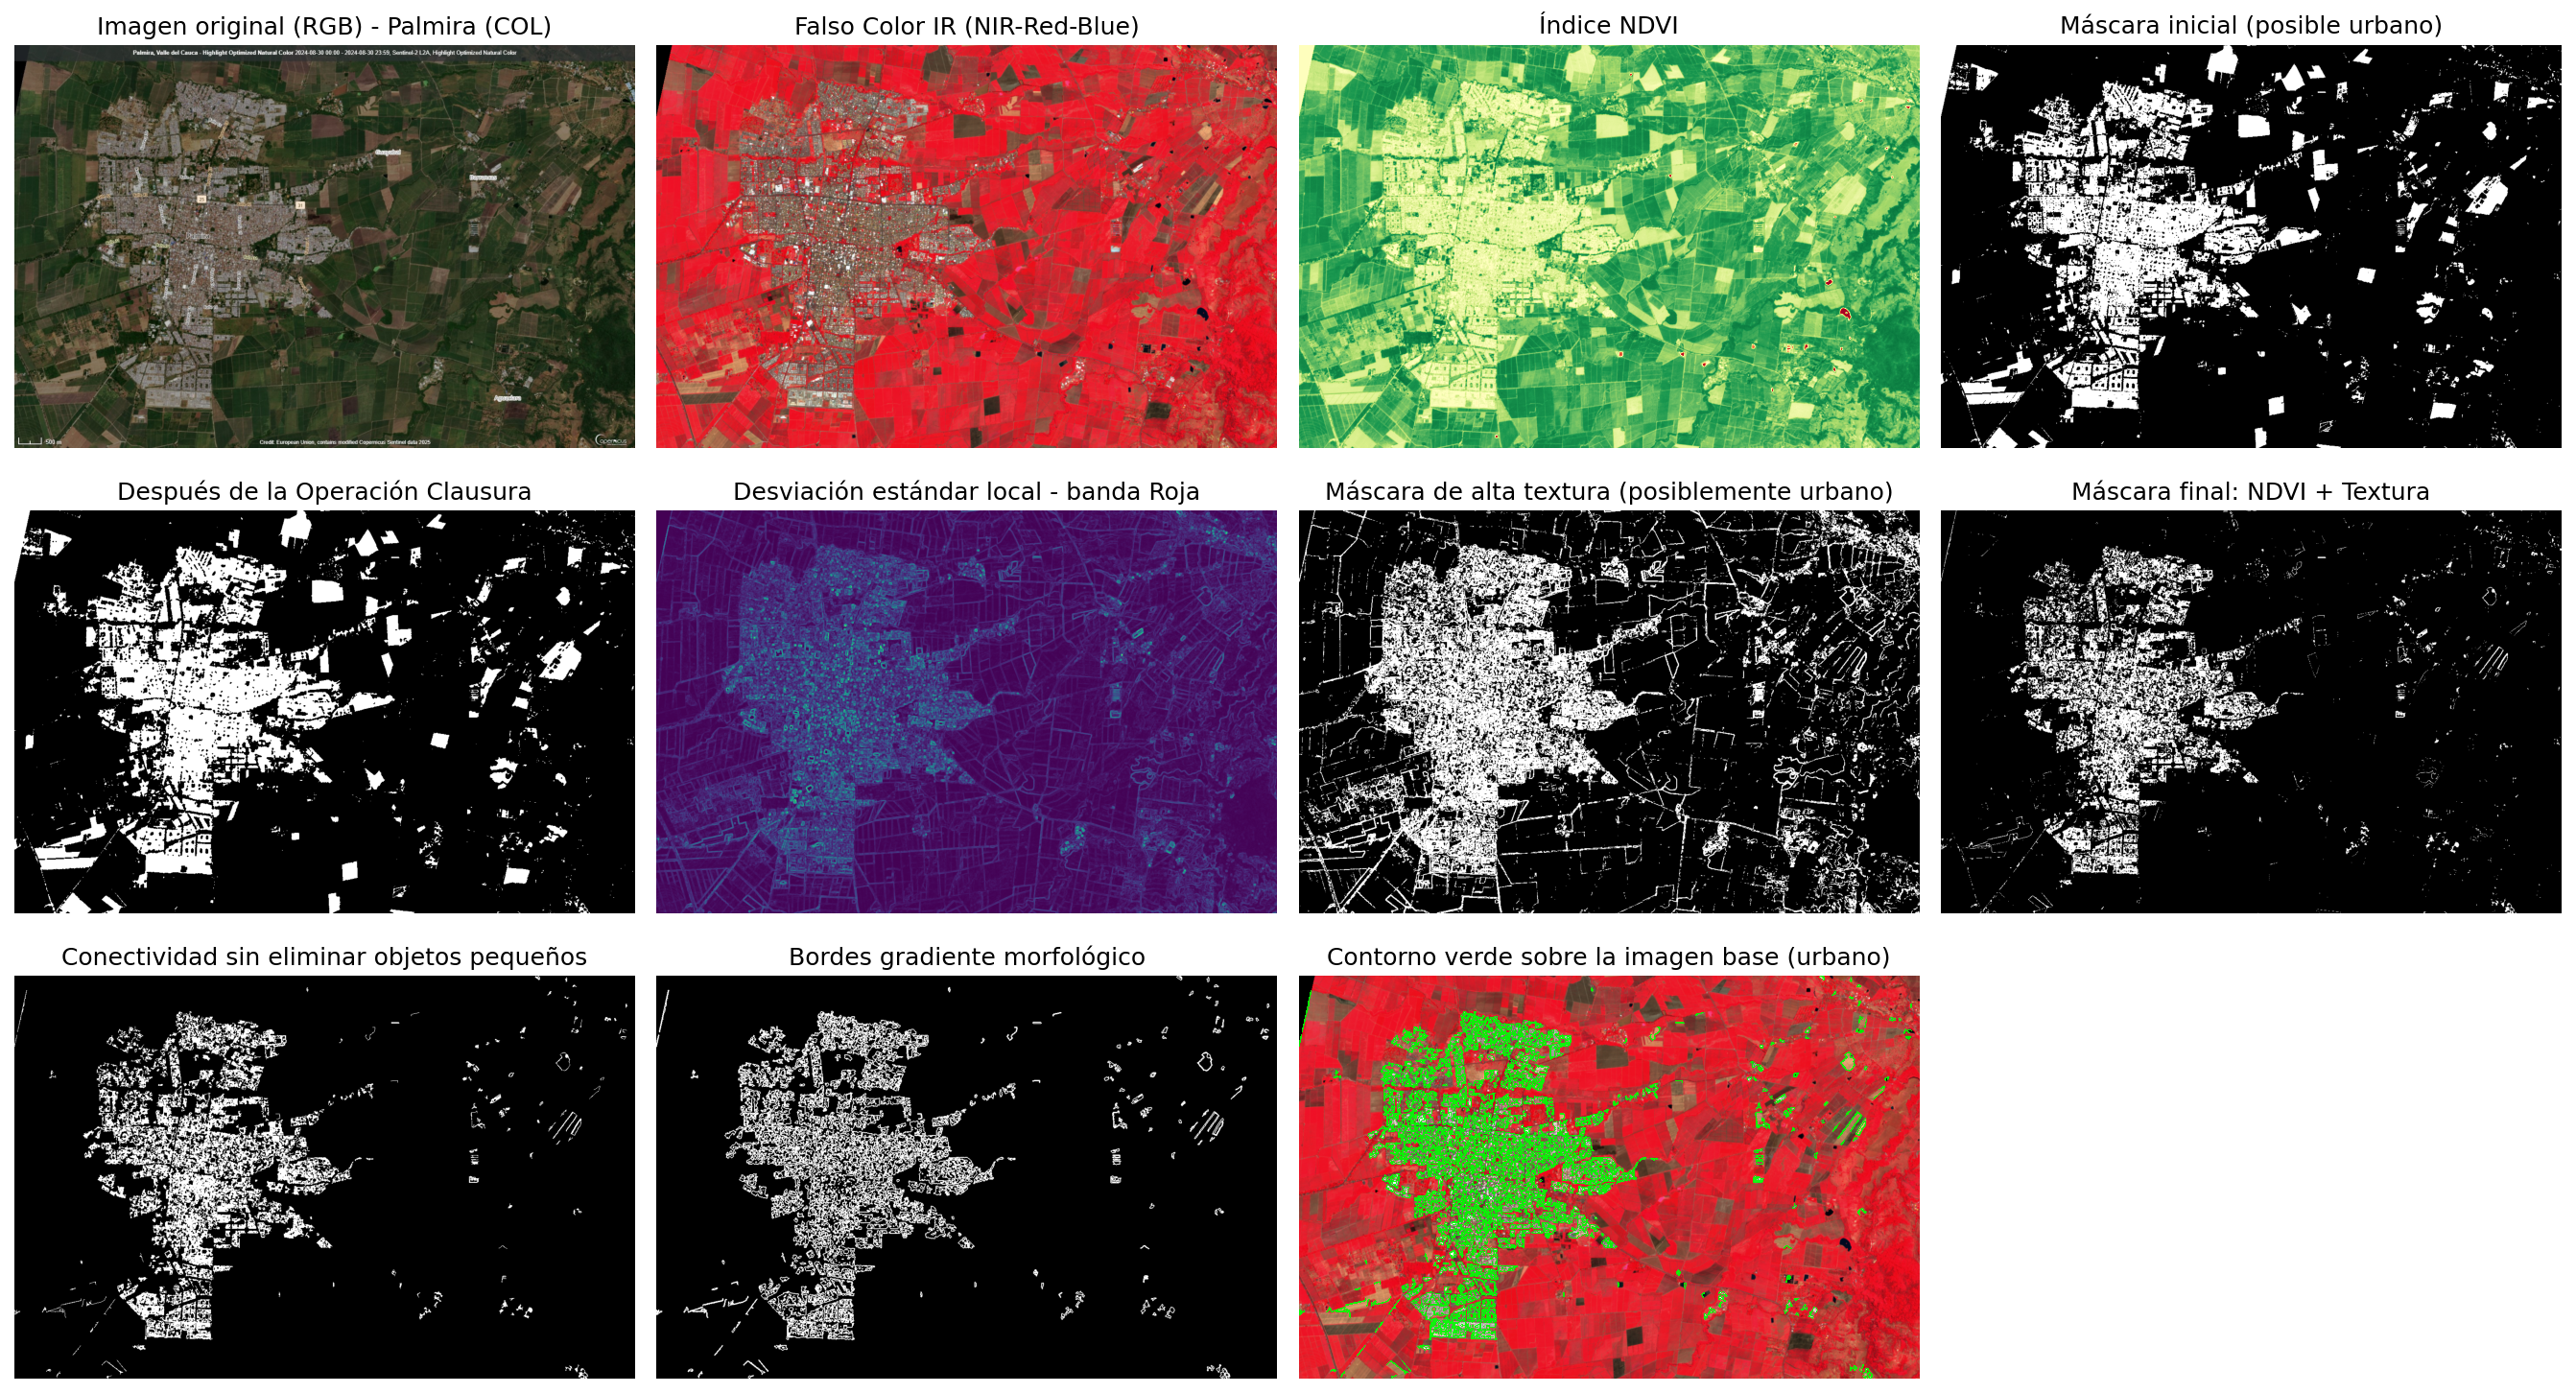
\includegraphics[height=0.3\textwidth]{./figures/drive/Procesado_Imagen_satelital_Palmira.png}
    \caption{Resultados de la detección de zonas urbanas en imágenes NIR-R-B.}
    \label{fig:palmira_results}
\end{figure*}

\begin{figure*}[t]
    \centering
    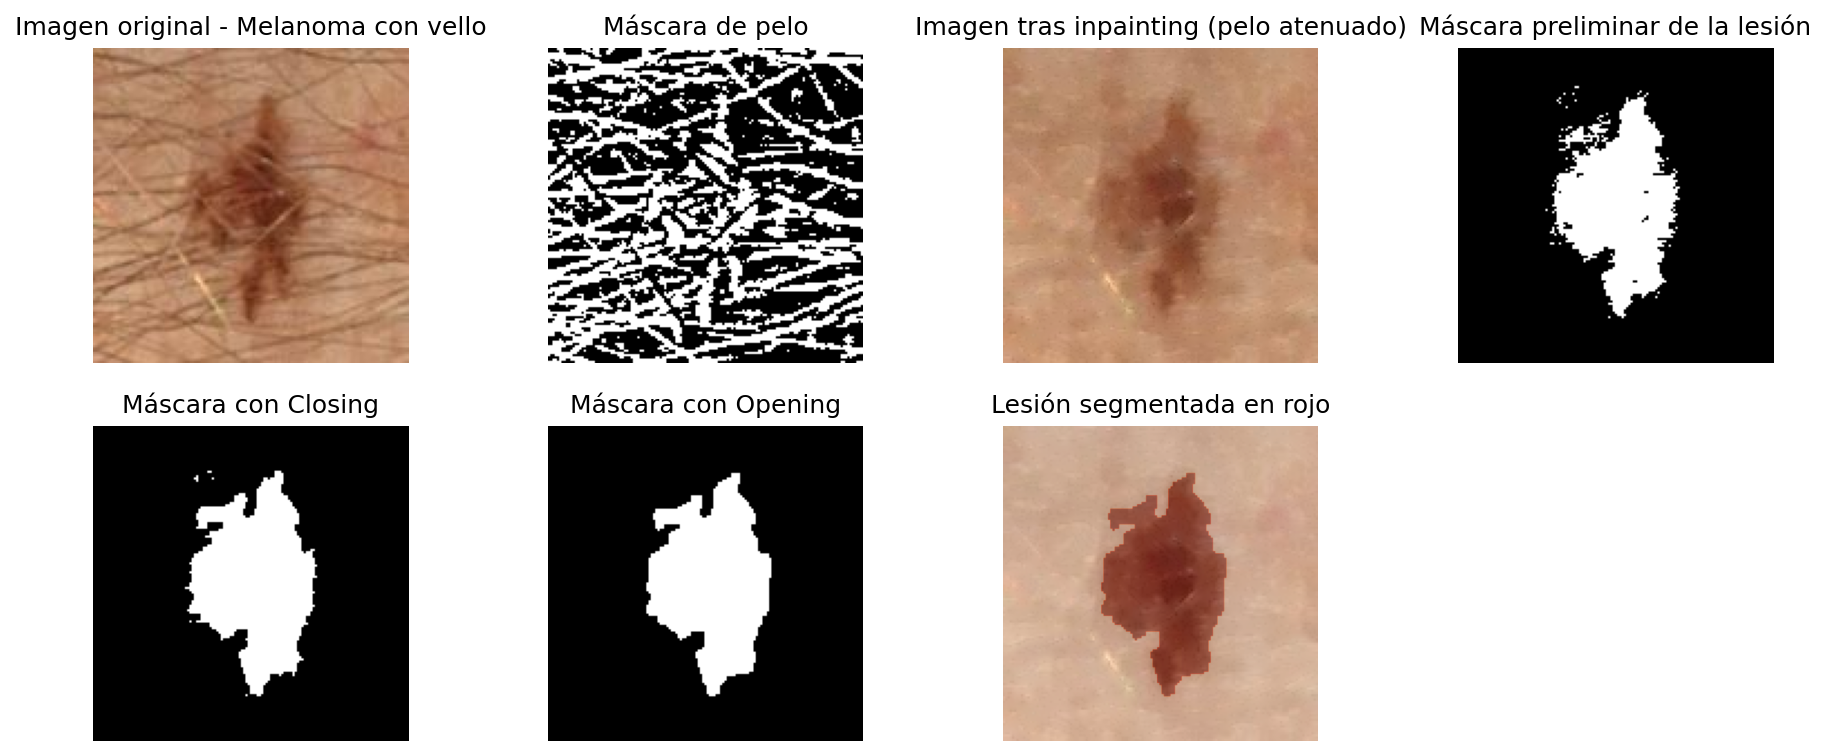
\includegraphics[height=0.3\textwidth]{figures/drive/Procesado_Imagen_Melanoma.png}
    \caption{Resultados de la segmentación de melanoma.}
    \label{fig:melanoma_results}
\end{figure*}
\section{Resultados y discusión}
% LTeX: language=es
\paragraph{Detección de Incendios Forestales} Los resultados de aplicar las transformaciones a la detección de incendios forestales se visualizan en la Figura \ref{fig:incendio_results}.

Cabe resaltar la importancia del incremento de contraste para resaltar los detalles del humo y del fuego, lo que facilita la detección de los contornos. La aplicación de operaciones morfológicas adicionales, como la dilatación y la eliminación de contornos secundarios, contribuye a mejorar la calidad de la detección y a reducir el ruido en la imagen procesada y posterior detección de la ubicación del incendio.

La fusión de la imagen original con el contorno dilatado proporciona una representación visual intuitiva del objeto de interés, lo que facilita la interpretación de los resultados. \\

\paragraph{Detección de Retinopatía Diabética} Los resultados de aplicar las transformaciones a la detección de retinopatía diabética se visualizan en la Figura \ref{fig:retinopatia_results}.

El método propuesto logra resaltar eficazmente las áreas de potencial daño vascular asociadas a la retinopatía diabética. La detección de bordes y el procesamiento morfológico permiten identificar regiones sospechosas, mientras que la ecualización del histograma mejora significativamente el contraste y la visibilidad de los detalles vasculares. Es importante recalcar como la aplicación de la operación
de apertura permite filtrar el ruido y centrar la atención en las áreas de interés de geometría similar al kernel utilizado.\\

\paragraph{Inspección de Calidad en Frutas} Los resultados de aplicar las transformaciones a la inspección de calidad en frutas se visualizan en la Figura \ref{fig:frutas_results}.


Se evidencia claramente como la aplicación del operador de Sobel en ambas direcciones permite resaltar los bordes de las frutas, lo que facilita la detección de defectos. No obstante, es un caso particular para el tomate pues es una fruta lisa. Este metodo podría no funcionar con frutas con presencia natural de imperfecciones, para lo cual se debería utilizar otro acercamiento.\\

\paragraph{Detección de Automóviles en parqueadero} Los resultados de aplicar las transformaciones a la detección de automóviles en un parqueadero se visualizan en la Figura \ref{fig:parqueadero_results}.


Se observa claramente como la aplicación de operadores morfológicos y espaciales permite aislar los automóviles en el parqueadero y remover ruido como algunos árboles, sombras y las líneas de parqueo. No obstante, al realizar la detección de bordes con Canny y encontrar los contornos, se siguen observando bordes no pertenecientes a automóviles. Esto podría mejorarse mediante la aplicación de un filtro que tome únicamente los contornos con aproximaciones a un cuadrado.\\

\paragraph{Detección de orillas en puertos} Los resultados de aplicar las transformaciones a la detección de orillas en puertos se visualizan en la Figura \ref{fig:puerto_results}.

Se observa que las imágenes poseen una gran diferencia desentendiendo de la tonalidad de grises con las que son binarizadas. En este caso, se observa como al utilizar un mayor umbral para la binarización (bordes 2), se logra tener una definición mucho mayor de los bordes al aplicar el operador de Sobel. A su vez, se observa también las diferencias entre ambos métodos utilizados de eliminación de barcos. En este caso, es mucho más eficiente el método por áreas ante el método de apertura, en donde la imagen pierde su forma y su interpretación es pobre en comparación a la imagen en donde se filtran los barcos por áreas.

Esto se debe a la propia contextualización de la imagen, donde la superficie no es un elemento continuo al ser escala de grises. Está representado por una multiplicidad de objetos menores. En el caso del método de apertura, está aplicada de forma homogénea a toda la imagen. Sin embargo, el método de reconocimiento de áreas busca una superficie adecuada al valor seleccionado, permitiendo así que los barcos (rodeados de agua y claramente delineados) posean una superficie menor a lo pautado y, consecuentemente, sean removidos.\\

\paragraph{Detección de Tumores Cerebrales} Los resultados de aplicar las transformaciones a la detección de tumores cerebrales se visualizan en la Figura \ref{fig:tumor_results}.

Se observa la particularización del tumor con respecto a la imagen original, así como la limpieza de ruido como resultado de los operadores morfológicos y espaciales. Se observa como la operación de apertura tiene el efecto de eliminar pequeños objetos o protuberancias que podrían haber sido introducidos por la dilatación inicial, suavizar los contornos del tumor, eliminando irregularidades menores.

\paragraph{Detección de defectos en pantallas de celulares} Los resultados de aplicar las transformaciones a la detección de defectos en pantallas de celulares se visualizan en la Figura \ref{fig:celular_results}.

A partir de la imagen original, se genera la conversión de la imagen a blanco y negro. Luego, por medio de la erosión, se intenta la eliminación de las marcas. Se observa que la eliminación no es total, pero si reducida en un buen porcentaje. Esto se genera para poder implementar el proceso de Top-hat, como lo marca la imagen final. Gracias a esto, se permite resaltar las diferencias y poder vislumbrar las marcas con mayor rigor. El proceso, en este caso, incluye la eliminación de la marca en conjunto con la diferencia entre imágenes para poder realizar de forma genérica la visualización de las marcas propias de todos los posibles celulares.

Es importante recalcar que como los bordes del celular también poseen la misma forma de línea que las marcas, son objeto de remoción al aplicar la erosión, por lo cual la imagen final muestra que los bordes del celular son altamente visibles, entendiendo así que no es el mejor método para esta aplicación, o se requiera de métodos adicionales de recorte o aislamiento anteriores a la aplicación de las transformaciones.


\paragraph{Detección de Zonas Urbanas en Imágenes NIR-R-B}

Los resultados del análisis de la imagen satelital NIR-RB para la detección de la huella urbana de Palmira se muestran en la Figura  \ref{fig:palmira_results}. Se evidencia una segmentación efectiva de las áreas urbanizadas. El proceso de composición de falso color infrarrojo, utilizando las bandas NIR, roja y azul, resaltó claramente la diferencia entre las zonas urbanas y la vegetación circundante. La aplicación del índice NDVI fue crucial para distinguir entre áreas con vegetación y potenciales zonas urbanas, proporcionando una base sólida para la segmentación inicial.

El análisis de textura, basado en la desviación estándar local de la banda roja, demostró ser particularmente efectivo para diferenciar entre áreas urbanas y suelos desnudos o campos cosechados, que inicialmente podrían confundirse con zonas urbanizadas. La combinación de las máscaras NDVI y de textura, seguida de un filtrado por conectividad, resultó en una delimitación precisa de la huella urbana, incluyendo tanto el núcleo urbano principal como asentamientos más pequeños en las áreas periféricas.

La visualización final, que superpone los bordes detectados sobre la imagen original, muestra una clara demarcación de las áreas urbanizadas. Se observa una buena correspondencia con la estructura urbana visible en la imagen de color natural, validando la efectividad del método. Notablemente, el algoritmo logró detectar no solo el área urbana principal de Palmira, sino también pequeños asentamientos y estructuras dispersas en las zonas rurales circundantes, demostrando su sensibilidad a diferentes escalas de urbanización.

Sin embargo, se notaron algunas limitaciones, como la inclusión de algunas áreas de cultivo seco que fueron detectadas erróneamente como zonas urbanas debido a su alta textura. A pesar de esto, el método demostró ser robusto en su capacidad para distinguir la mayoría de las áreas urbanizadas de su entorno rural, proporcionando una herramienta valiosa para el análisis urbano y la planificación territorial en la región de Palmira.



\paragraph{Detección de Melanoma}

Los resultados de la segmentación del melanoma se muestran en la Figura \ref{fig:melanoma_results}. Se logra una identificación precisa y efectiva de la lesión en la imagen dermatológica. El proceso de eliminación del vello mediante Black-hat e inpainting proporcionó una base limpia para el análisis. 

La segmentación inicial utilizando el canal de luminosidad del espacio HSV, seguida de refinamientos morfológicos, produjo una máscara bien definida del melanoma. La imagen final muestra una superposición precisa de la segmentación sobre la lesión original, capturando con fidelidad la forma irregular del melanoma, sus bordes bien definidos y las variaciones de color y textura internas. La exclusión efectiva de la piel sana circundante y la preservación de detalles importantes de la lesión demuestran la robustez del método.
\section{Conclusiones}
% LTeX: language=es
Este estudio ha demostrado la continua relevancia y eficacia de los filtros espaciales y morfológicos en diversas aplicaciones de procesamiento de imágenes. Los resultados obtenidos en la detección de tumores cerebrales, identificación de defectos en pantallas de celulares, detección de zonas urbanas en imágenes satelitales y segmentación de melanomas son particularmente prometedores. 

La capacidad de estas técnicas para delimitar con precisión áreas de interés, como la huella urbana en imágenes satelitales o la forma irregular de melanomas en imágenes dermatológicas, subraya su utilidad en escenarios complejos. Aunque se observaron algunas limitaciones, como la ocasional clasificación errónea en imágenes satelitales, el rendimiento general de estos métodos fue robusto y efectivo. 

Este trabajo resalta el valor persistente de los enfoques clásicos de procesamiento de imágenes, que pueden complementar eficazmente las técnicas más modernas como el aprendizaje profundo. Se recomienda continuar la investigación para refinar estas técnicas y explorar su integración con métodos más avanzados, lo que podría conducir a soluciones aún más potentes en el campo del análisis y procesamiento de imágenes.







\newpage
\section{Referencias}
\printbibliography[heading=none]
\newpage
\end{document} 